\documentclass{beamer}

\usepackage[utf8]{inputenc}
\usepackage[T1]{fontenc}
\usepackage{graphicx}
\usepackage{hyperref}

\title{Image Embedding for Product Labeling}
\author{Couture Vision}
\date{\today}

\begin{document}

\frame{\titlepage}

\section{Project Objective}
\begin{frame}{Project Objective}

\textbf{Goal:}
\begin{itemize}
    \item Based on a photo of an article, match the reference image of this article.
\end{itemize}

\textbf{Example:}
\begin{columns}
    \column{0.5\textwidth}
    \begin{figure}[t]
        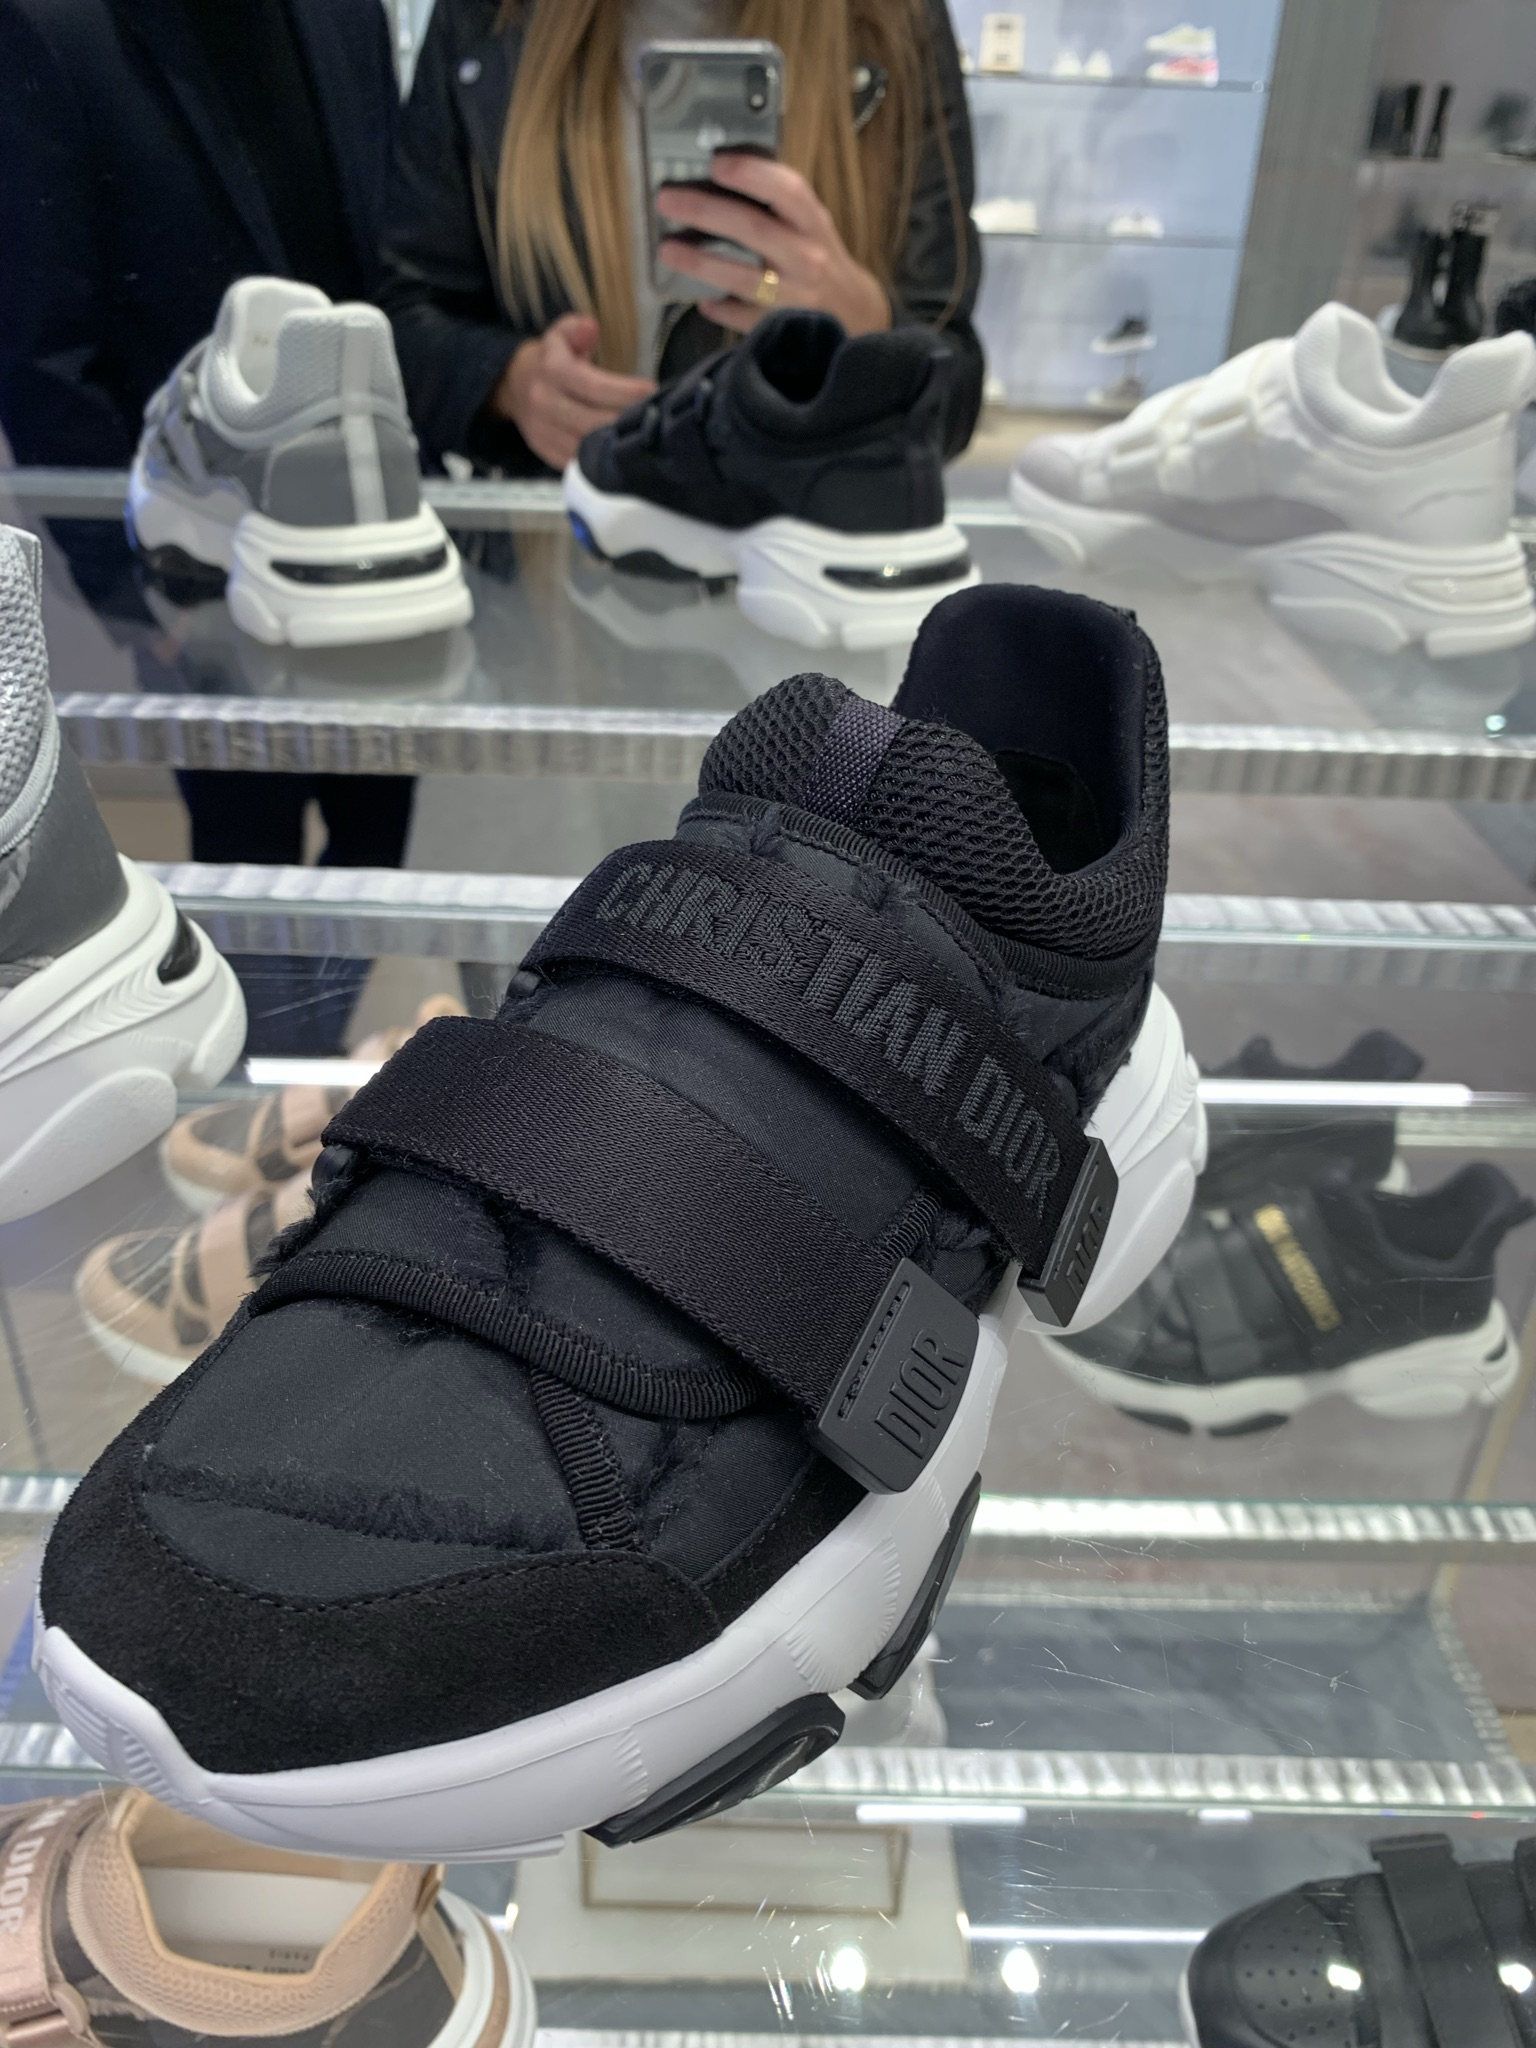
\includegraphics[width=0.6\textwidth]{assets/shoe_test.jpg}
        \caption{Test Image}
    \end{figure}
    \column{0.5\textwidth}
    \begin{figure}[t]
        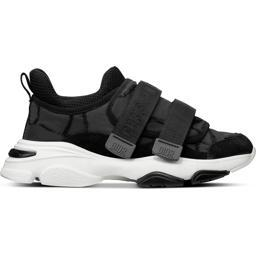
\includegraphics[width=0.6\textwidth]{assets/shoe_reference.jpeg}
        \caption{Reference Image}
    \end{figure}
\end{columns}

\end{frame}

\begin{frame}{Test set labeling}
    \begin{itemize}
        \item We labeled the test set manually, using embeddings to suggest potential matches.
        \item The test set contains 80 images.
        \item Some items don't have a corresponding image in the DAM.
        \item Some items are very similar to others, making classification challenging.
    \end{itemize}
    \begin{columns}
        \column{0.5\textwidth}
        \begin{figure}
            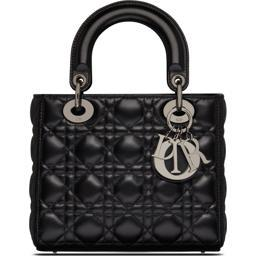
\includegraphics[width=0.65\textwidth]{assets/very_similar_items_1.jpeg}
            \caption{Black bag}
        \end{figure}
        \column{0.5\textwidth}
        \begin{figure}
            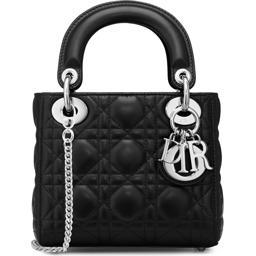
\includegraphics[width=0.65\textwidth]{assets/very_similar_items_2.jpeg}
            \caption{Another black bag}
        \end{figure}
    \end{columns}
\end{frame}


\section{Introduction}
\begin{frame}{Project Overview}
\begin{itemize}
    \item We tried a lot of models to extract embeddings: Microsoft's ResNet50, Google's ViT Patch-16, OpenAI's CLIP, Meta's DINOv2 and ViTMSN.
    \item Cosine similarity is used to find the best matches between images. Better than Euclidean distance. We also tried a mix of both.
    \item We replaced \texttt{rembg} background removal by \texttt{RMBG 2.0}.
    \item All images were cropped and zoomed to the object.
    \begin{columns}
        \column{0.5\textwidth}
        \begin{figure}
            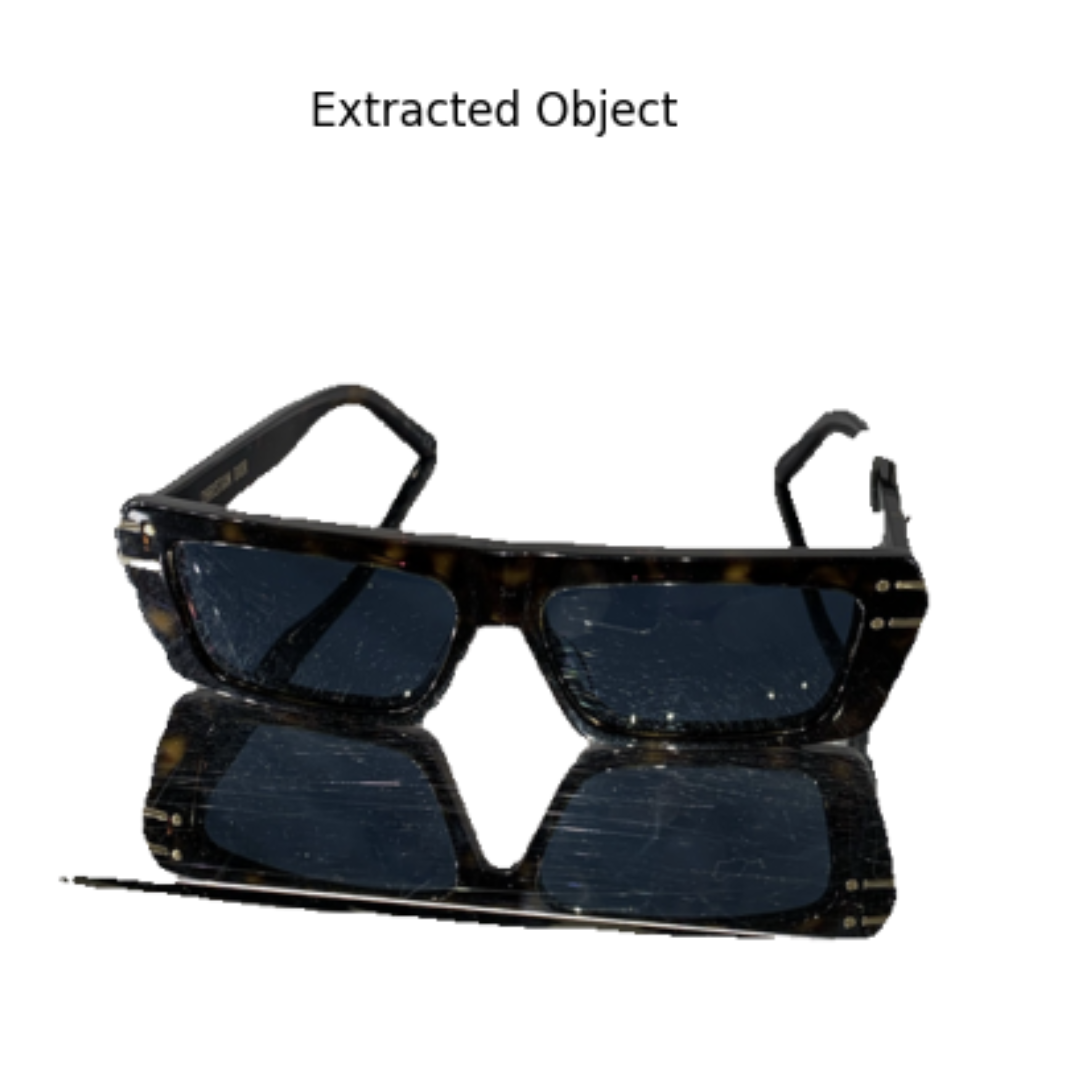
\includegraphics[width=0.5\textwidth]{assets/glasses_rembg.png}
            \caption{Background removal using \texttt{rembg}}
        \end{figure}
        \column{0.5\textwidth}
        \begin{figure}
            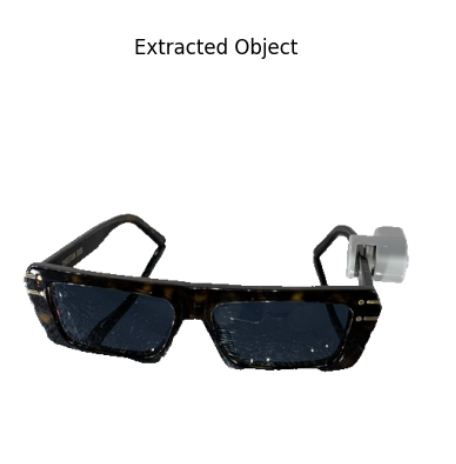
\includegraphics[width=0.5\textwidth]{assets/glasses_rmbg_2.png}
            \caption{Background removal using \texttt{RMBG 2.0}}
        \end{figure}
    \end{columns}
\end{itemize}
\end{frame}

\begin{frame}{Data augmentation with a 3D generation model}
    \begin{itemize}
        \item We used \textbf{TRELLIS} for generating 3D models for the 2700 DAM assets.
        \item We used \textbf{Blender} to render the 3D models in 8 different angles each.
    \end{itemize}
    
    \begin{columns}
        \column{0.5\textwidth}
        \begin{figure}
            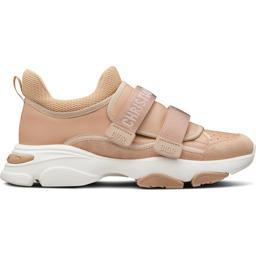
\includegraphics[width=0.65\textwidth]{assets/trellis_input.png}
            \caption{Input for TRELLIS}
        \end{figure}
        \column{0.5\textwidth}
        \begin{figure}
            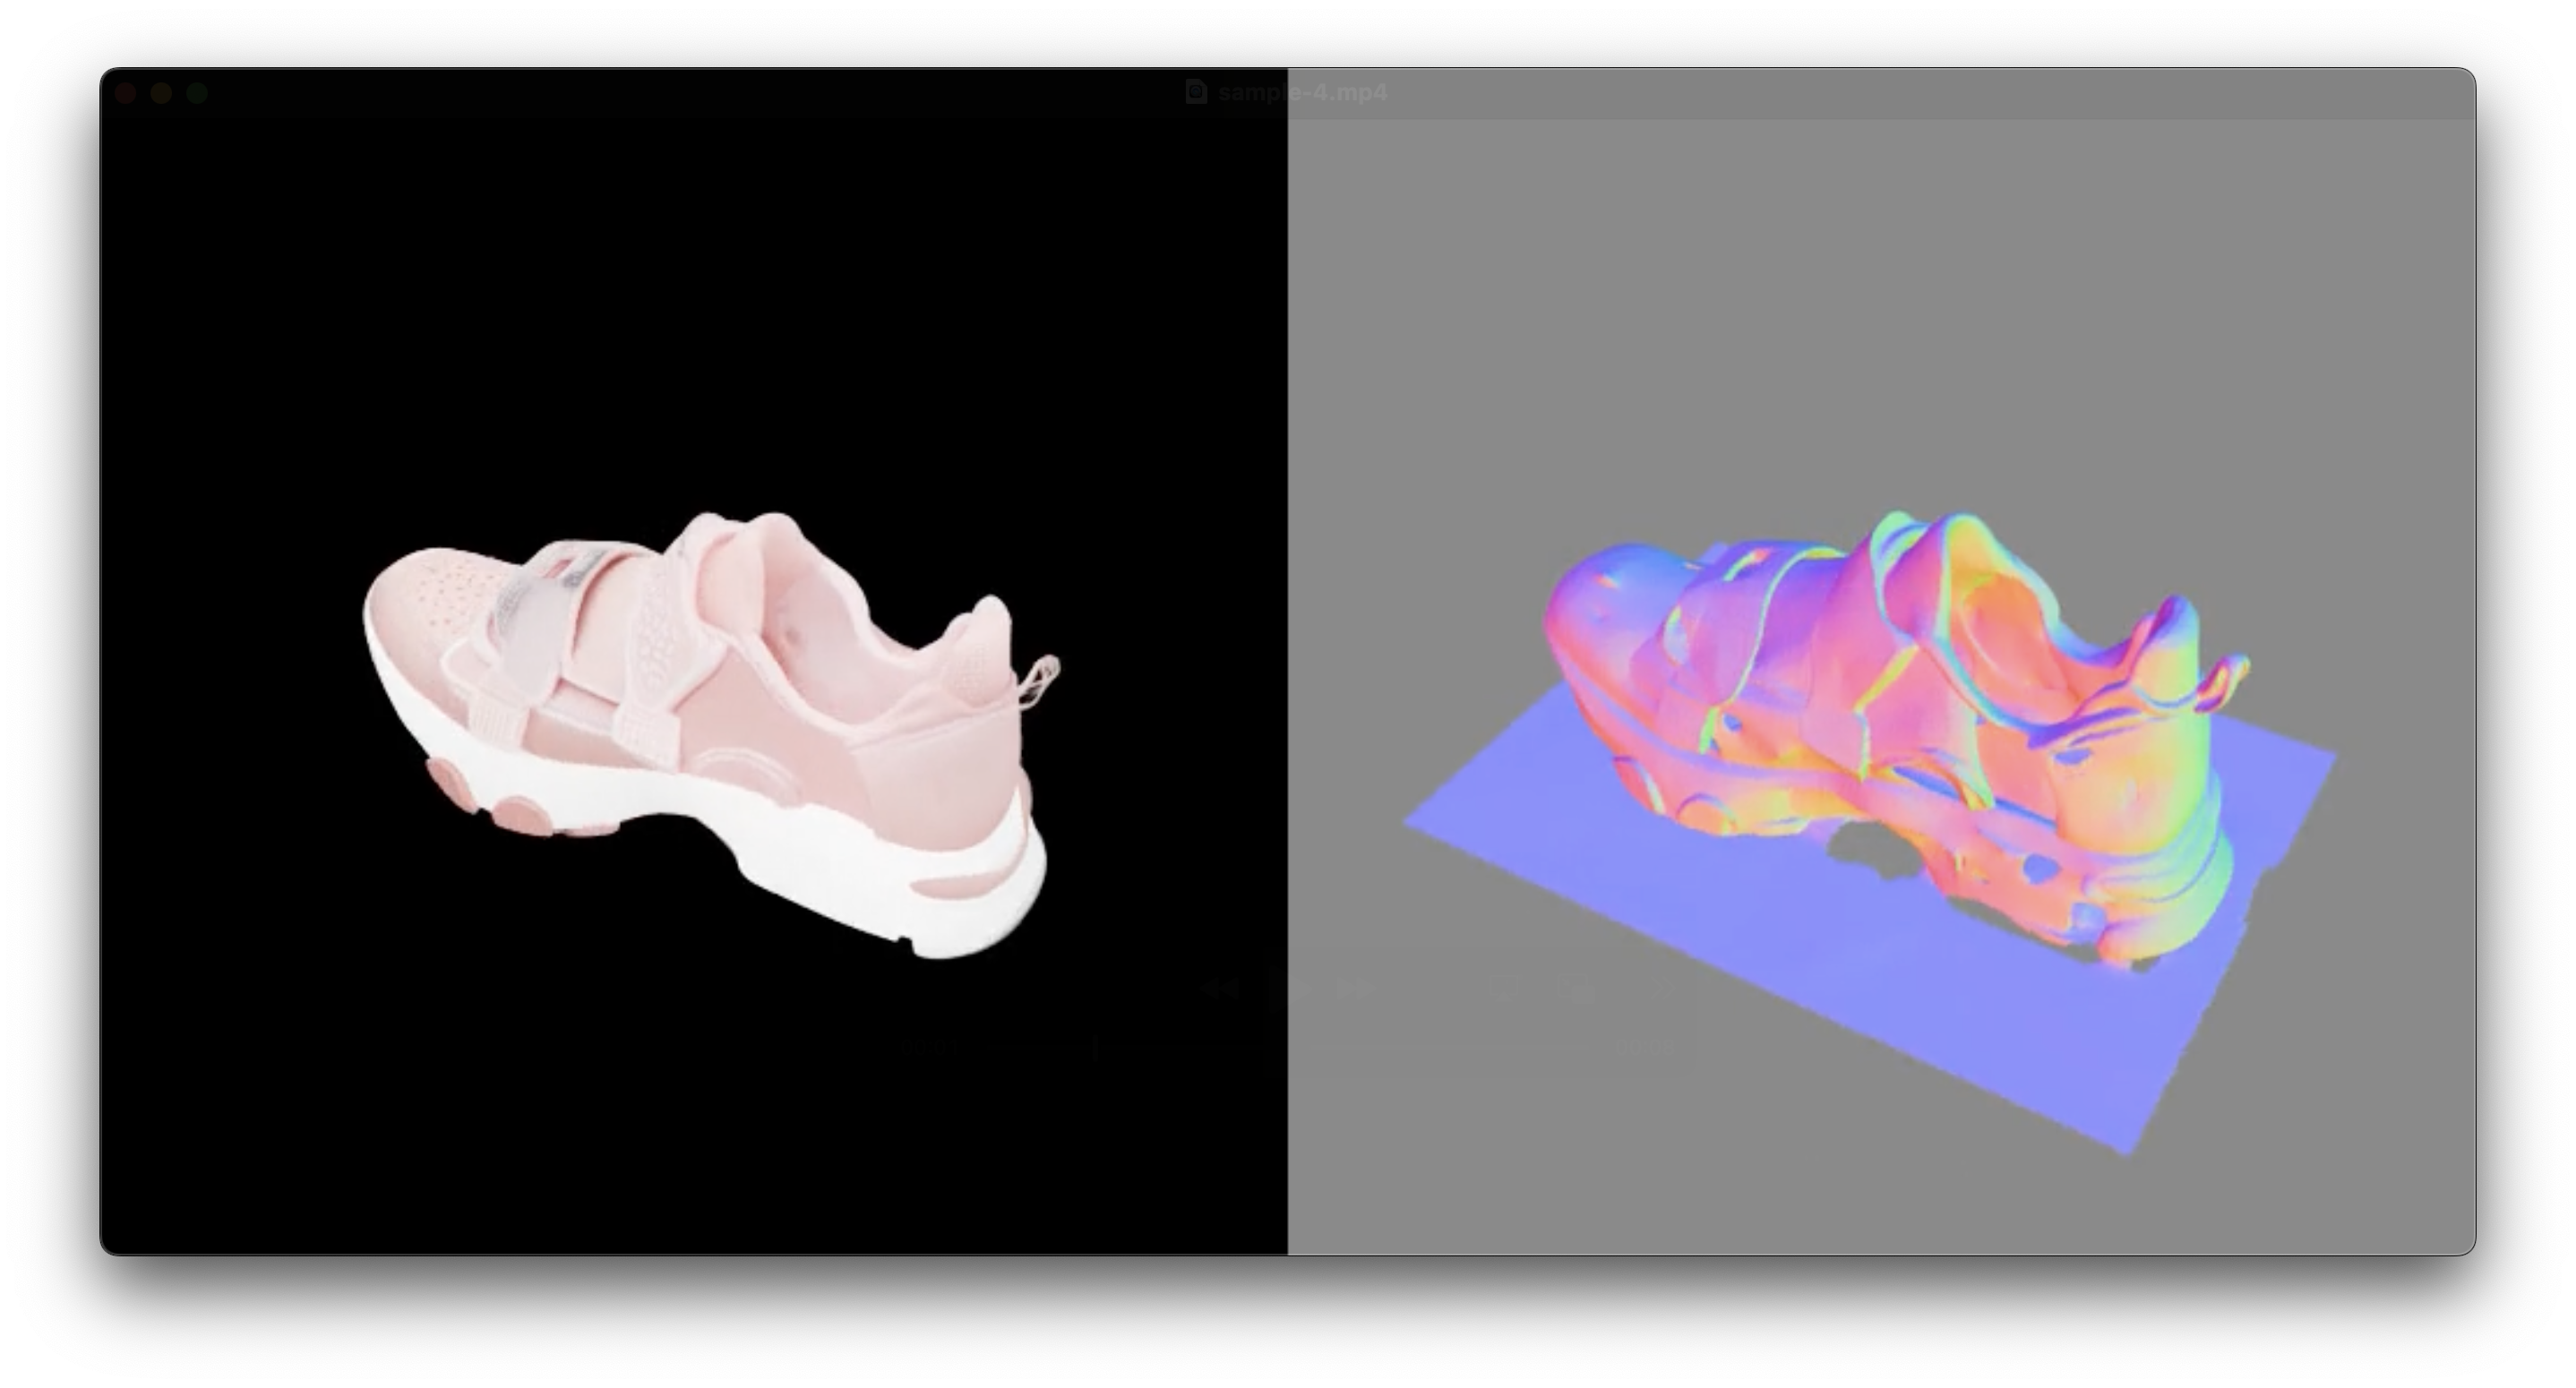
\includegraphics[width=1\textwidth]{assets/trellis_output.png}
            \caption{TRELLIS generated 3D model}
        \end{figure}
    \end{columns}
    
\end{frame}

\begin{frame}{Data augmentation with a 3D generation model}
    % 4 images, 2x2
    \begin{figure}
        \centering
        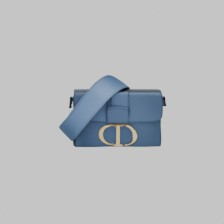
\includegraphics[width=0.35\textwidth]{assets/M9204UMOSM49E-1.jpeg}
        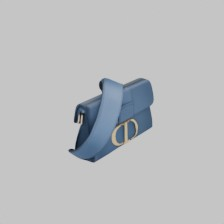
\includegraphics[width=0.35\textwidth]{assets/M9204UMOSM49E-2.jpeg}
        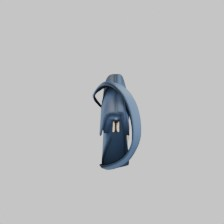
\includegraphics[width=0.35\textwidth]{assets/M9204UMOSM49E-3.jpeg}
        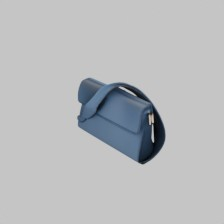
\includegraphics[width=0.35\textwidth]{assets/M9204UMOSM49E-4.jpeg}
        \caption{3D renders of a bag}
    \end{figure}
\end{frame}

\begin{frame}{The performance improvements}
    \begin{itemize}
        \item Adding embeddings of the 3D renders improved the Top-1 performance from 36\% to 42\%.
        \item Averaging 2D and 3D embeddings improved the Top-1 performance from 42\% to 52\%.
        \item We then removed all 2D embeddings and only used 3D embeddings, which improved the Top-1 performance from 52\% to 56\%.
        \item We used gradient descent on 25\% of the test set to tune the weights for merging 2D and 3D embeddings, as well as the feature selection weights, which improved the Top-1 performance from 56\% to 61\%.
        \item Final results: Top-1: 61\%, Top-3: 79\%, Top-5: 84\%.
    \end{itemize}
\end{frame}

\section{User Interface}
\begin{frame}{Web Interface with Gradio}
\begin{itemize}
    \item Develop a simple UI using Gradio.
    \item Users can upload a picture and get top-X matches.
    \item The UI will display the reference DAM image with its ID, the top-X matches, and a 3D render of the item.
\end{itemize}
\end{frame}

\section{NLP Approach}
    \begin{frame}{Using NLP for Image-to-Text and Matching}
    \begin{itemize}
        \item \textbf{Image-to-Text Conversion}:
        \begin{itemize}
            \item Generate descriptive captions for images to capture key attributes like color, material, and unique features.
        \end{itemize}
        \item \textbf{Text Embedding and Matching}:
        \begin{itemize}
            \item Convert captions into embeddings and store them in a vector database.
            \item Perform similarity search to find the closest matches to client-uploaded images.
        \end{itemize}
        \item \textbf{Combination with Image Embeddings}:
        \begin{itemize}
            \item This approach can be enhanced by combining text-based embeddings with image-based embeddings for improved accuracy.
        \end{itemize}
    \end{itemize}
\end{frame}

\begin{frame}{Improvement Attempt Using NLP}
    There are some challenging cases, with \textbf{color} or \textbf{texture}:
    \vspace{0.5cm} % Ajouter un espace vertical

    % Ajouter deux images côte à côte
% Ajouter une image à gauche et une description à droite
    \centering
    \begin{minipage}{0.5\textwidth}
        \centering
        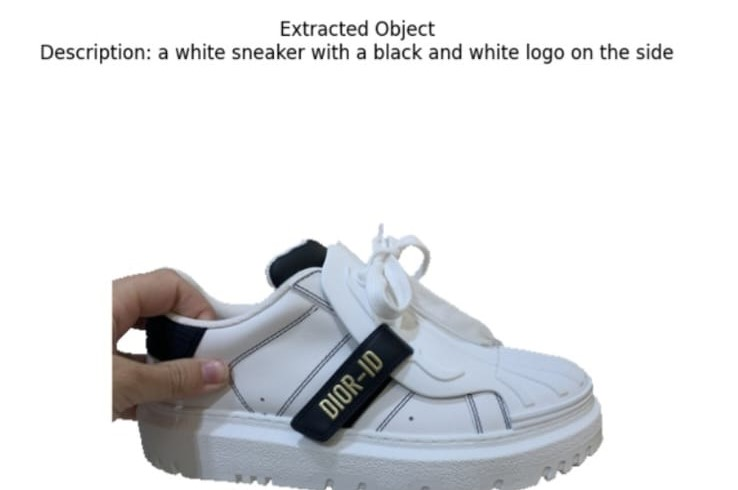
\includegraphics[width=\textwidth]{assets/wrongColorShoes.jpg}
    \begin{figure}[h]
        \caption{Example: Color mismatch}
    \end{figure}
    \end{minipage}
    \hfill
    \begin{minipage}{0.45\textwidth}
        \raggedright
        \textbf{Blip Description:}
        \vspace{0.3cm} % Espacement entre le titre et la description
        \textit{"A white sneaker with a black and white logo on the side"}
    \end{minipage}
\end{frame}

\begin{frame}{Using NLP for Image-to-Text and Matching}

Steps : 
    \vspace{0.5cm} % Ajouter un espace vertical
    \begin{enumerate}
        \item Generate descriptions using the \textbf{BLIP model}.
        \item Convert descriptions into \textbf{text embeddings}.
        \item Combine \textbf{text embeddings} with 2D image embeddings and 3D-rendered image embeddings
        \item Use the \textbf{mean embedding} for improved matching.
    \end{enumerate}
\end{frame}

% Slide 3: Refining Results with Modern NLP Techniques
\section{Refining Results}
\begin{frame}{Improving Top-1 result}
    \begin{itemize}
        \item Use \textbf{more recent BLIP models} for better descriptions.
        \item Question prompt:
            \begin{quote}
                What is the object in this image? What is its color? What is its texture? What is a specific detail about it? \\
                Answer in the format: [object, color, texture, specificity].
            \end{quote}
        \end{itemize}

    \vspace{0.5cm}
    \textbf{Proposed Method}
    \begin{itemize}
        \item Select the top-5 DAM candidates selected after applying the cosine similarity on the embedding (without the BLIP embedding). 
        \item Apply BLIP to the top-5 and the test image to generate a structured description.
        \item Keep the candidate with the \textbf{highest overlap} in responses with the test image.
        \end{itemize}
\end{frame}

\end{document}
